\chapter{Erprobung der Navigation}
In diesem Kapitel werden die Ergebnisse der zuvor diskutierten Algorithmen in realen Anwendungsszenarien untersucht. Als Beispiel dient der Laborraum F001 der Hochschule Karlsruhe, von dem im Voraus eine Karte mithilfe des ROS-Pakets \lstinline{hector_slam}{} aufgezeichnet wurde. An dieser Stelle werden drei verschiedene Anwendungsfälle untersucht. Im Ersten wurde der Raum im Vergleich zur Karte nicht verändert. Außerdem wird angenommen, dass die Position des Roboters zu Beginn der Navigation bekannt ist. Somit handelt es sich um den trivialsten Anwendungsfall der Navigation, womit die Grundfunktionen nachgewiesen werden sollen.
Im zweiten Szenario wird der Fall untersucht, das der auf der Karte unmittelbare Weg zum Ziel durch ein Hindernis blockiert wird, wodurch gezwungenermaßen Sensordaten beachtet werde müssen, um einen Weg zum Ziel zu planen.
Der letzte Test dient zur Beurteilung der Lokalisierung. In diesem Fall wird die Roboterposition als unbekannt angenommen und durch mittels einer ungenauen Schätzung initialisiert. 

\newpage
\section{Anwendungsszenario 1: Triviale Navigation}
Das erste Szenario dient auf der einen Seite dem Nachweis der Grundfunktionen der Navigation. Auf der anderen Seite wird das simple Beispiel genutzt, um die Bedienung und Auswertung des Experiment mittels \lstinline{RViz}{} zu erläutern. Den Ausgangspunkt aller Experimente stellt die  Karte des Labors dar, die unter Anderem in der folgenden Abbildung zu sehen ist. Die schwarzen Pixel stellen Hindernisse, die hellgrauen freie Flächen und die restlichen undefinierte Flächen dar.
\begin{figure}[!ht]
\centering
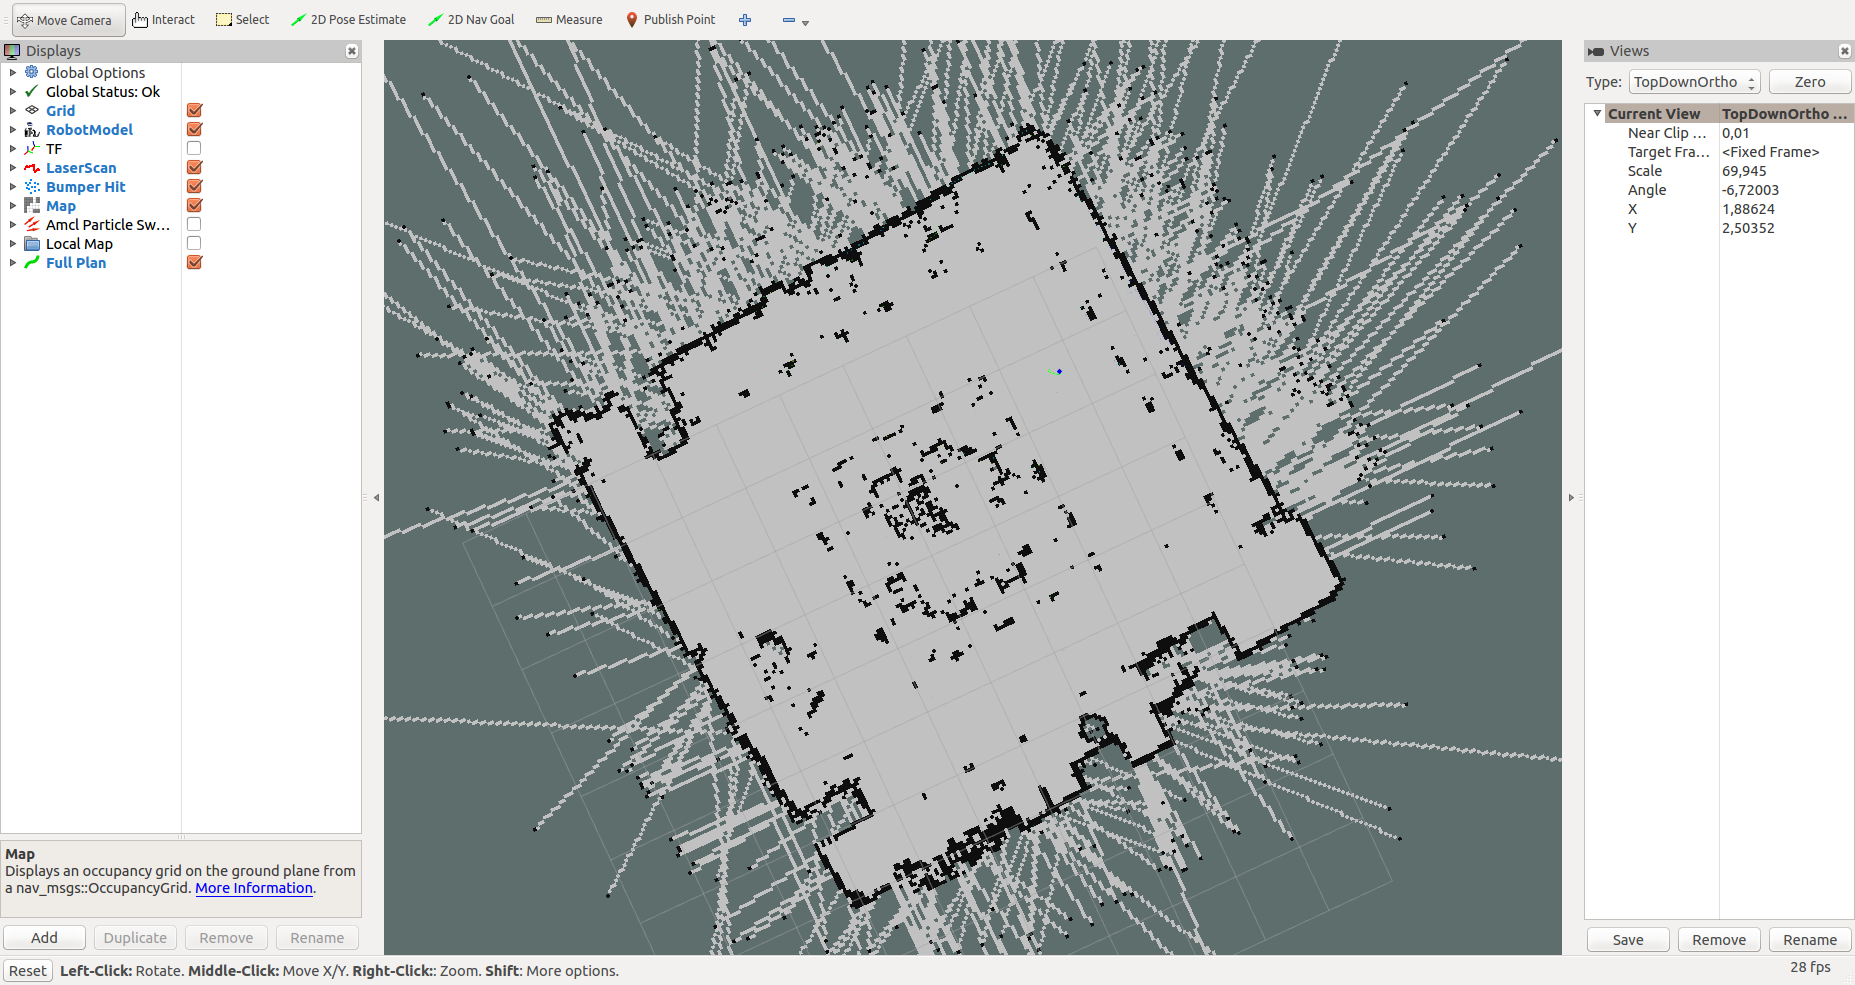
\includegraphics[width=0.8\linewidth]{img/Experiment1_RViz_Overview.png}
\caption{Übersicht von \lstinline{RViz}{}}
\end{figure}
Die Karte wird von \lstinline{RViz}{} angezeigt. Um die Visualisierung zu konfigurieren, können die Elemente auf der linken Seite nach Bedarf an- und abgewählt werden. In der Toolbar können die Elemente \lstinline{2D Pose Estimate}{} und \lstinline{2D Nav Goal}{} genutzt werden, um die eine Positionsschätzung anzugeben und das Ziel der Navigation anzugeben.
Mithilfe Letzteren wird ein Ziel in der entgegengesetzten Ecke des Raums vorgegeben, woraufhin ein globaler Pfad geplant wird, der in der folgenden Abbildung zu sehen ist.
\begin{figure}[!ht]
\centering
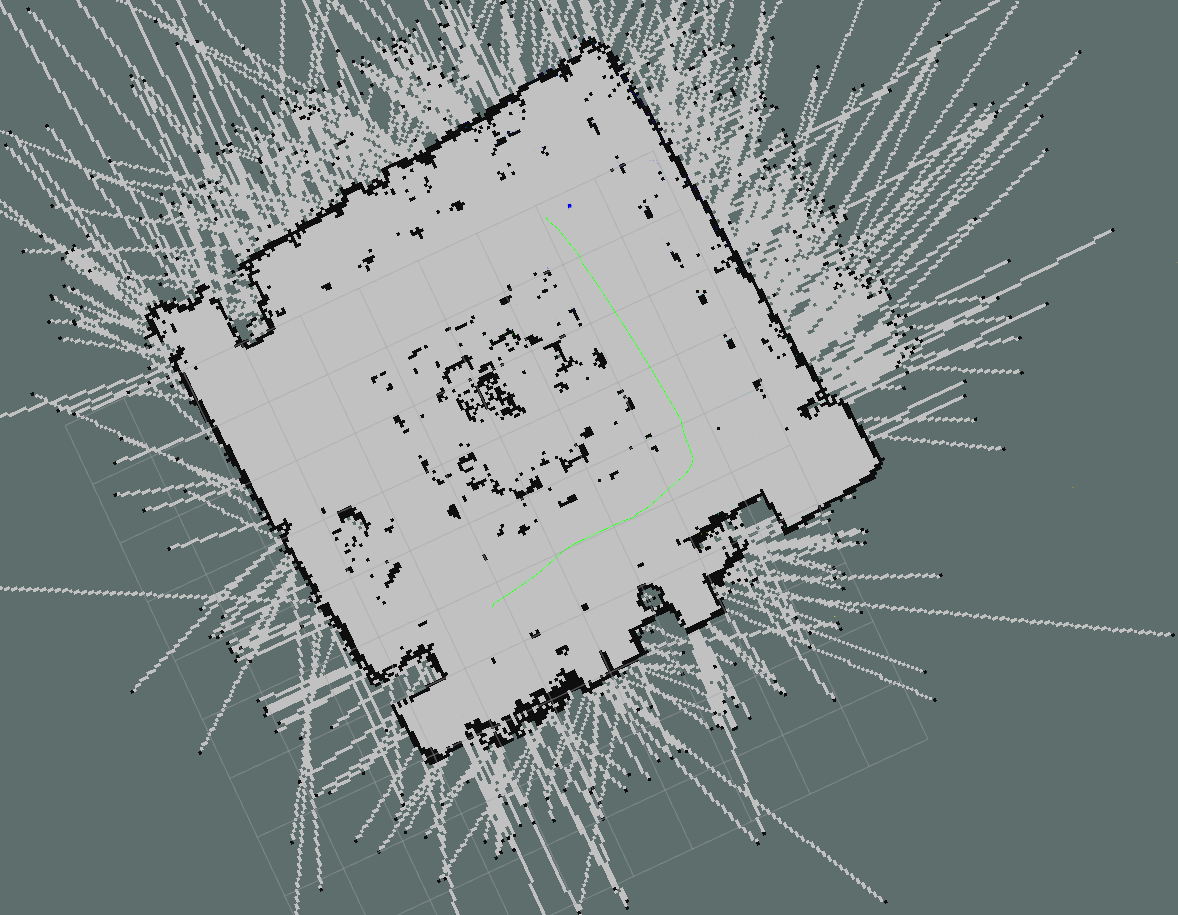
\includegraphics[scale=0.6, trim={7cm 6cm 9cm 3cm},clip]{img/Experiment1_Bild_Fullpath.png}
\caption{Globaler Plan}
\end{figure}

\newpage
Wie der oben eingezeichnete Pfad entsteht, wird recht leicht ersichtlich, wenn die globale Kostenkarte betrachtet wird. Die Bewertung der Zellen beginnt jeweils in den belegten Hindernissen und wird exponentiell fallend von diesen weg propagiert.
\begin{figure}[!ht]
\centering
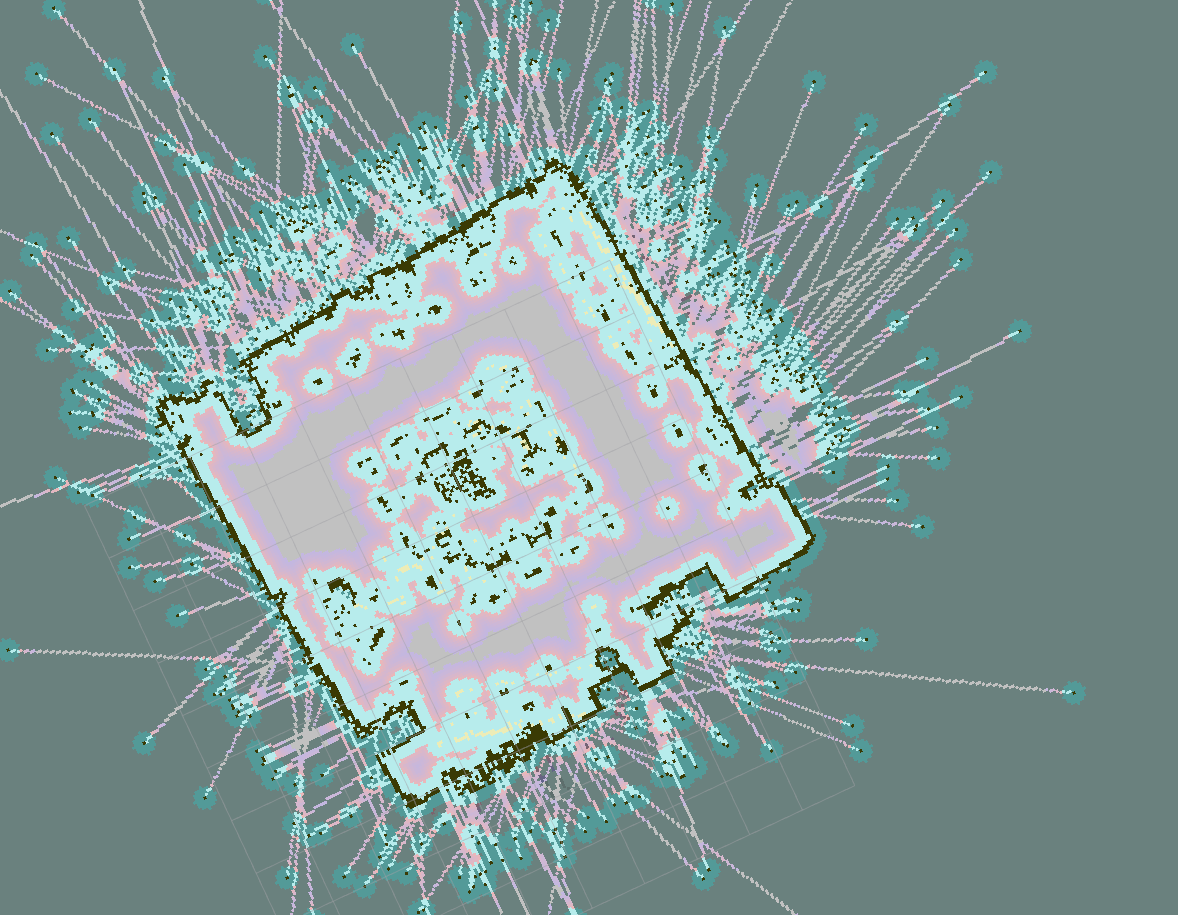
\includegraphics[scale=0.5, trim={4cm 2cm 9cm 3cm},clip]{img/Experiment1_Global_Costmap.png}
\caption{Globale Kostenkarte des Labors}
\end{figure}
Der gezeigt Pfade wurde nach der Planung problemlos von dem Roboter abgefahren, womit die Grundfunktion der Navigation nachgewiesen ist.

\newpage
\section{Anwendungsszenario 2: Hindernisdetektion}
Im nächsten Schritt wird der Fall betrachtet, dass der Weg des Roboters durch ein unbekanntes Hindernis versperrt wird. Darunter ist ein Objekt zu verstehen, dass bei der Kartenaufzeichnung nicht vorhanden war, weshalb der Roboter auf seine Sensordaten zurückgreifen muss, um den Gegenstand zu detektieren und in die Wegplanung einzuarbeiten. In der folgenden Abbildung sind die Position des Roboters als auch die aktuellen Sensordaten zu erkennen. An letzteren lässt sich die Position des Hindernisses deutlich erkennen.
\begin{figure}[!ht]
\centering
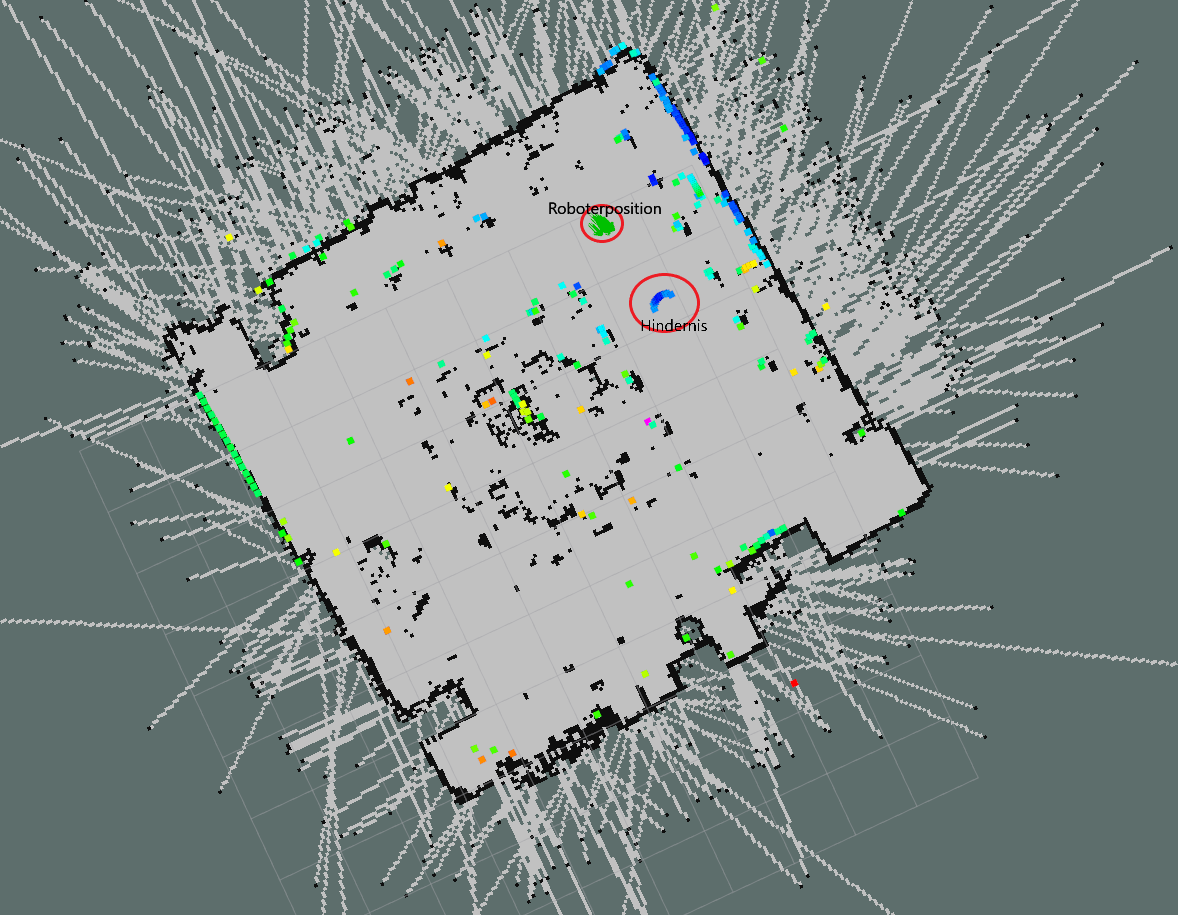
\includegraphics[scale=0.9,trim={13cm 13cm 9cm 2cm},clip]{img/Experiment2_Laserscan_Hindernis.png}
\caption{Roboter und Sensordaten mit Hindernis}
\end{figure}
\newpage
Die beiden weiteren Abbildungen zeigen wie die Sensordaten in die globale Kostenkarte integriert werden und wie daraufhin der globale Plan um die Distanzmessungen herumführt.
\begin{figure}[!ht]
\centering
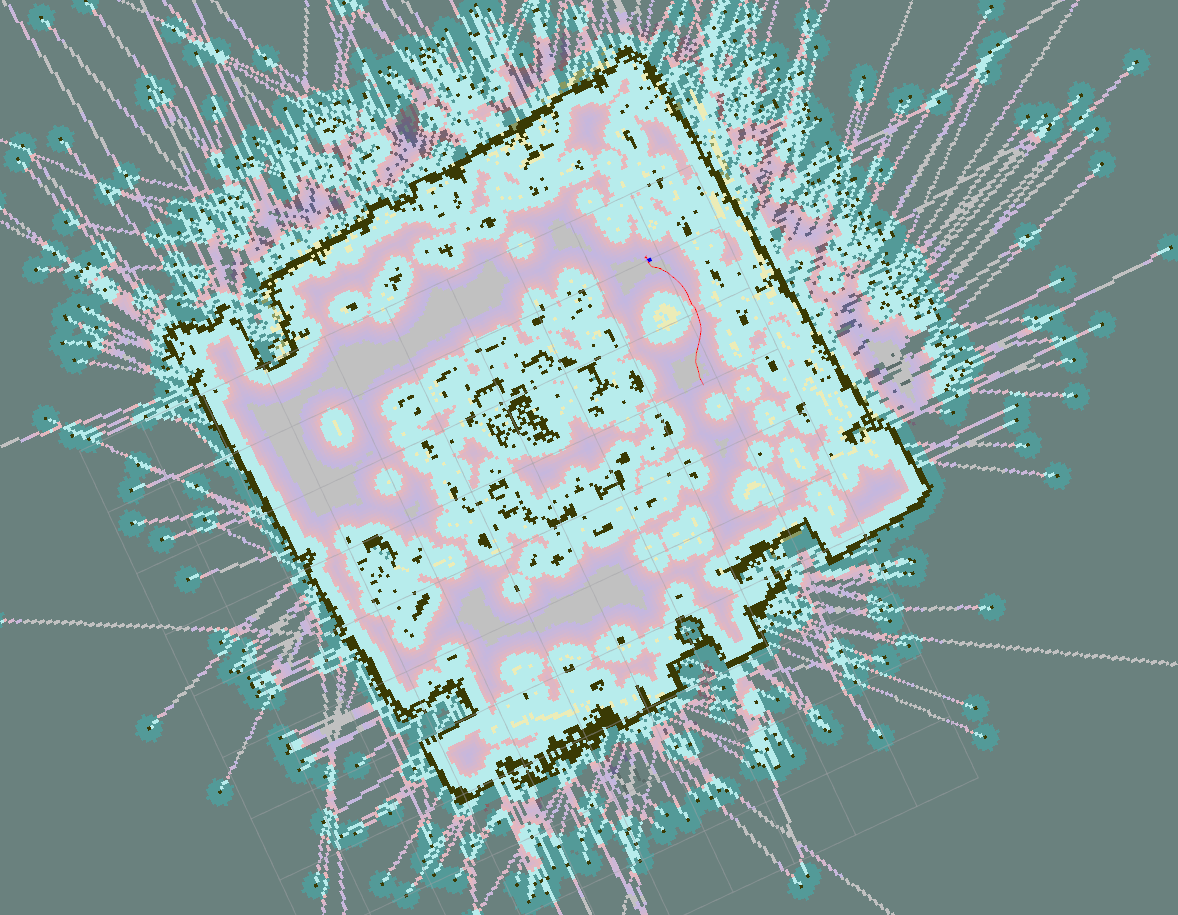
\includegraphics[width=0.45\linewidth ,trim={13cm 11cm 9cm 2cm},clip]{img/Experiment2_Global_Plan_Hindernis.png}
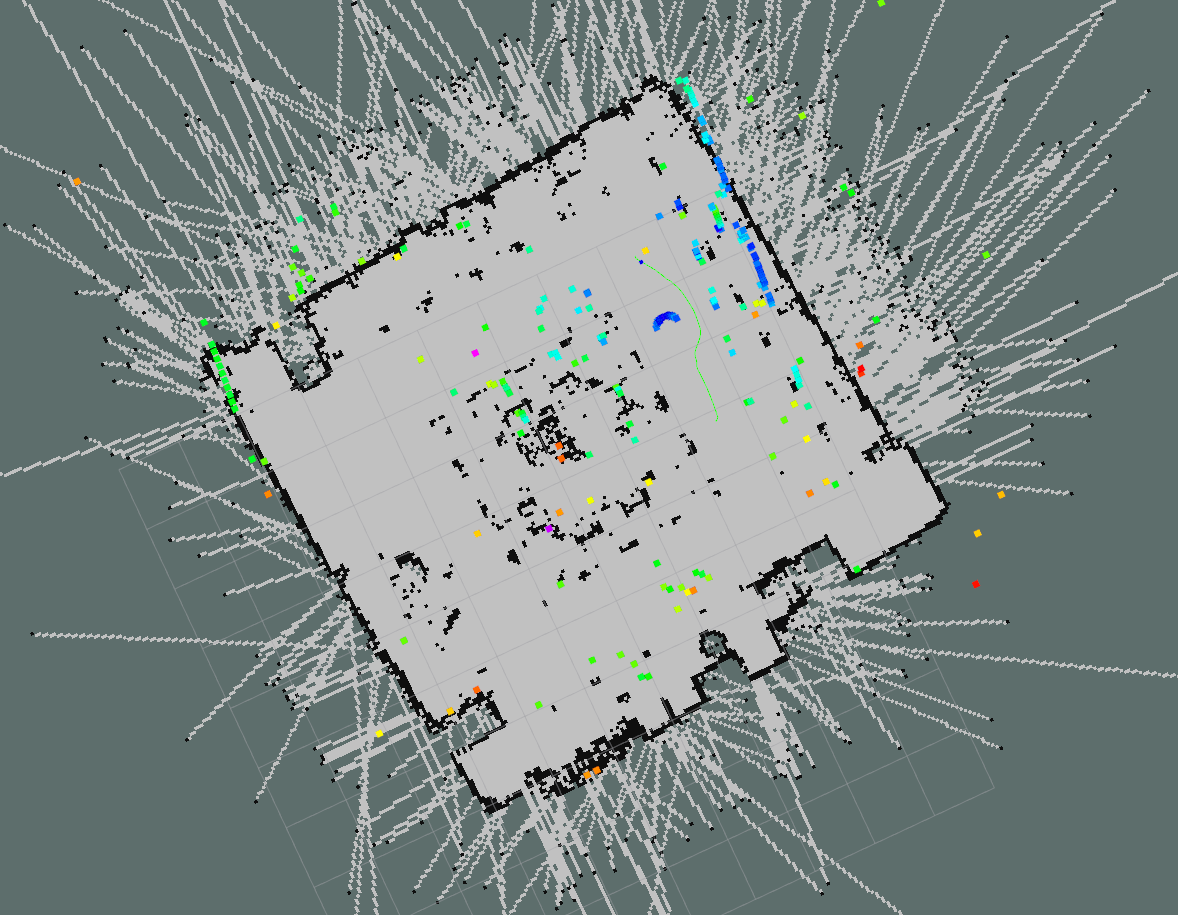
\includegraphics[width=0.45\linewidth ,trim={13cm 11cm 9cm 2cm},clip]{img/Experiment2_Global_Plan_Lascerscan_Hindernis.png}
\caption{Integration der Sensordaten in die Pfadplanung}
\end{figure}

In dem Experiment hat der Roboter das Hindernis nicht nur erfolgreich erkannt und in die Planung aufgenommen, sondern konnte die Route auch abfahren. Allerdings wurde hierbei die Geschwindigkeit deutlich reduziert, was darauf zurückzuführen ist, dass der Plan nach wie vor durch suboptimale Zonen führt. Der Grund hierfür liegt darin, das keine alternative Route zum Ziel führt, was aber auch zur Folge hat, dass der lokale Planer die Geschwindigkeit des Roboters reduziert, um auf potentielle Kollisionen reagieren zu können.

\newpage
\section{Anwendungsszenario 3: Lokalisierung}
Im letzten Versuch soll die Performanz der AMC-Lokalisierung untersucht werden. Hierfür wird der Roboter an einer Position im Raum ausgesetzt, die der Navigation nur als fehlerbehaftete, ungenaue Schätzung übergeben wird. Das Partikelfilter der Lokalisierung wird durch eine Positionsschätzung zurückgesetzt, das heißt die Partikel werden neu gezogen, wobei die geschätzte Position als Mittelwert der mehrdimensionalen Normalverteilung verwendet wird. Die initiale Varianz wird als Parameter des Algorithmus festgelegt. Die folgende Abbildung zeigt diesen Ausgangszustand, wobei die grünen Pfeile die verschiedenen Partikel darstellen, die wiederum als mögliche Positionen des Roboters verstanden werden. Außerdem sind die aktuellen Sensorwerte im Verhältnis zum Mittelwert der Partikelwolke eingezeichnet. Aus dem Vergleich der Distanzmessungen und des Wandverlaufs in der Karte wird ersichtlich, wie die Positionsschätzung des Roboters angepasst werden muss, sodass die Sensordaten mit der Umgebung übereinstimmen.
\begin{figure}[!ht]
\centering
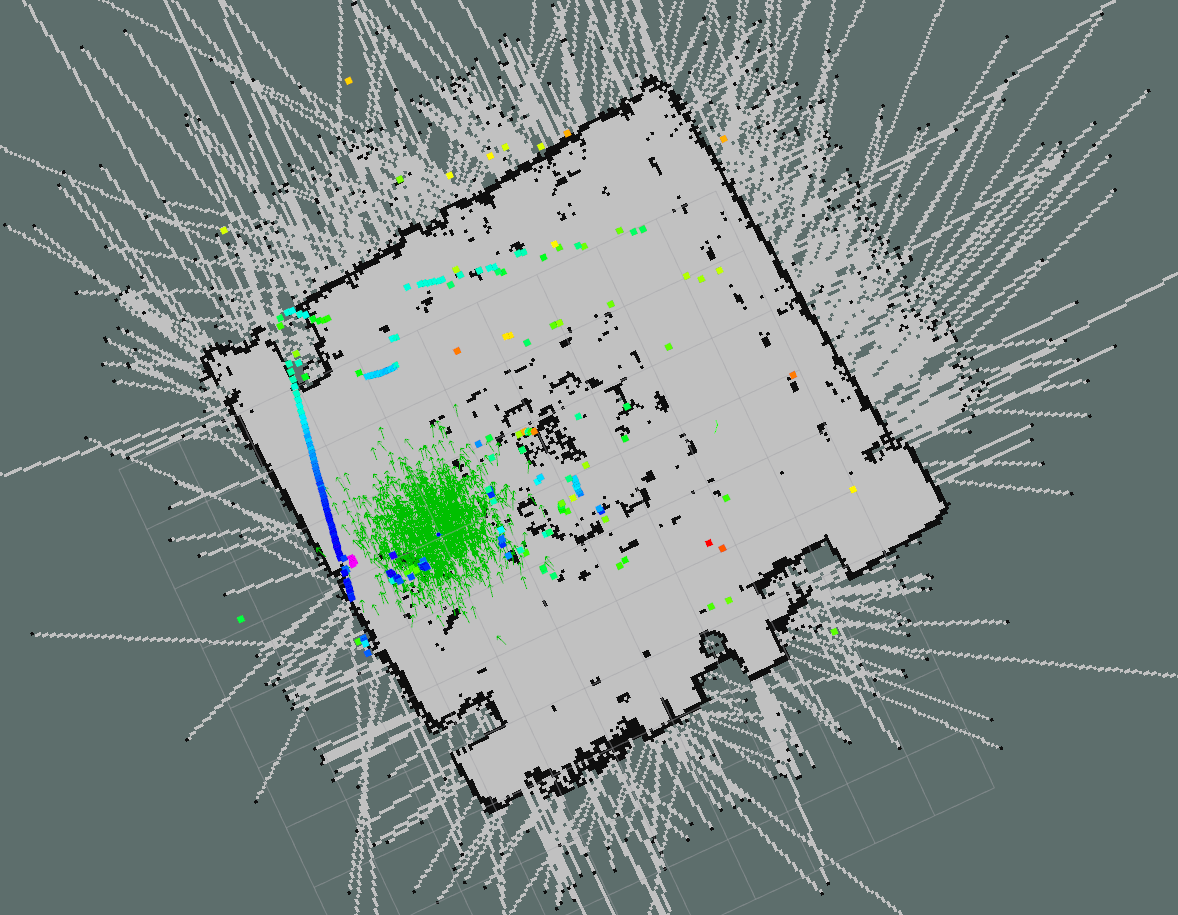
\includegraphics[width=0.7\linewidth, trim={4cm 5cm 12cm 6cm},clip]{img/Experiment3_Lokalisierung_1.png}
\caption{Ausgangszustand der Lokalisierung nach Positionsschätzung}
\end{figure}

Im nächsten Schritt der Navigation ein Zielpunkt in kurzer Distanz unmittelbar vor dem Roboter vorgegeben, woraufhin dieser die Bewegung startet. Während der Bewegung wird deutlich, dass sich der Mittelwert der Positionsschätzung verändert, was sich durch die Ausrichtung der Distanzmessungen zu dem Verlauf der Wände manifestiert. Dies zeigt sich in der nächsten Abbildung, wobei das Zusammenrücken der Partikel verdeutlicht, dass die Sicherheit der Lokalisierung zunimmt.
\begin{figure}[!ht]
\centering
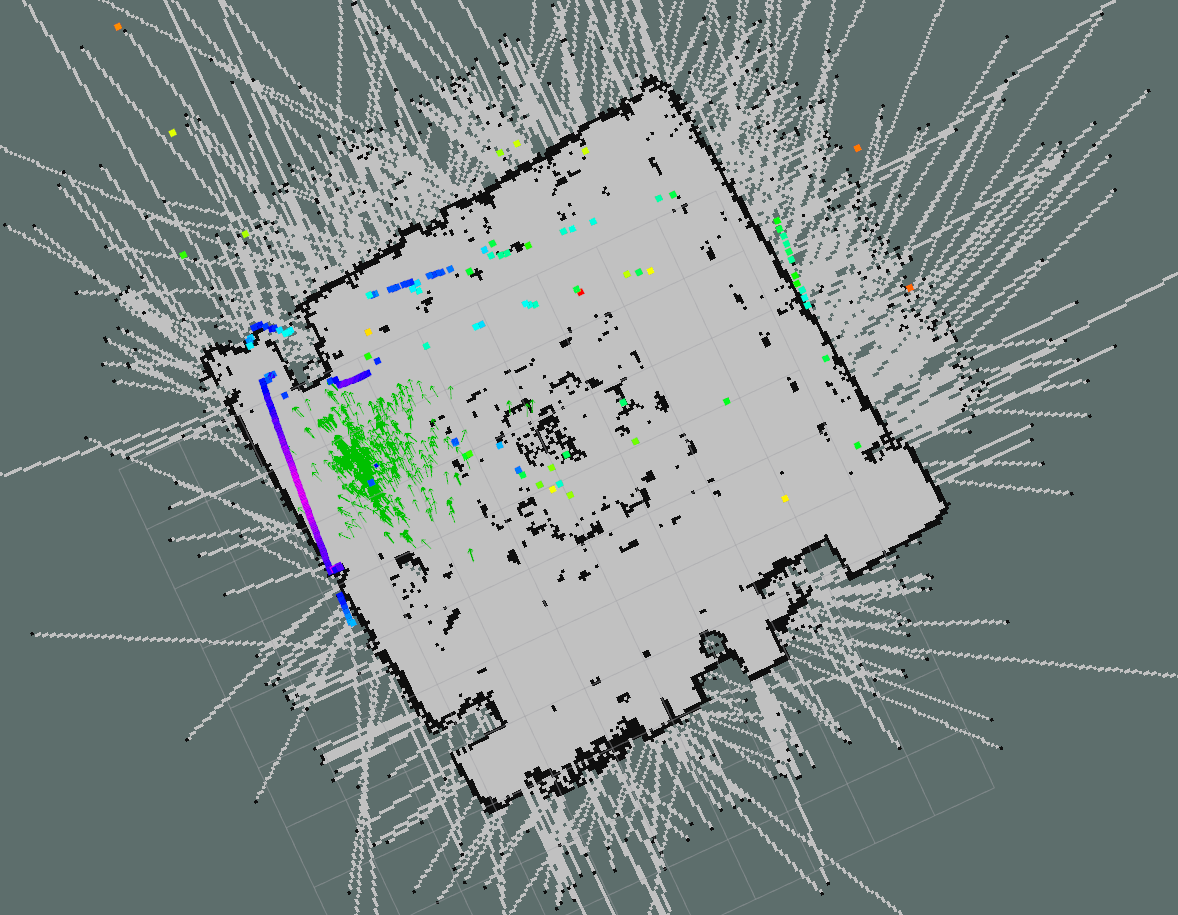
\includegraphics[width=0.7\linewidth, trim={4cm 5cm 12cm 6cm}, clip]{img/Experiment3_Lokalisierung_3.png}
\caption{Positionsschätzung nach kurzer Fahrdistanz}
\end{figure}

Die nächste Abbildung zeigt den Zustand der Lokalisierung in dem Moment, als der Zielpunkt erreicht wird. Nun stimmen die Punkte der Distanzmessung nahezu vollkommen mit den in der Karte eingezeichneten Hindernissen überein. Außerdem haben sich die Partikel weiter zusammengezogen, was für eine hohes Maß an Sicherheit der Lokalisierung spricht.
\begin{figure}[!ht]
\centering
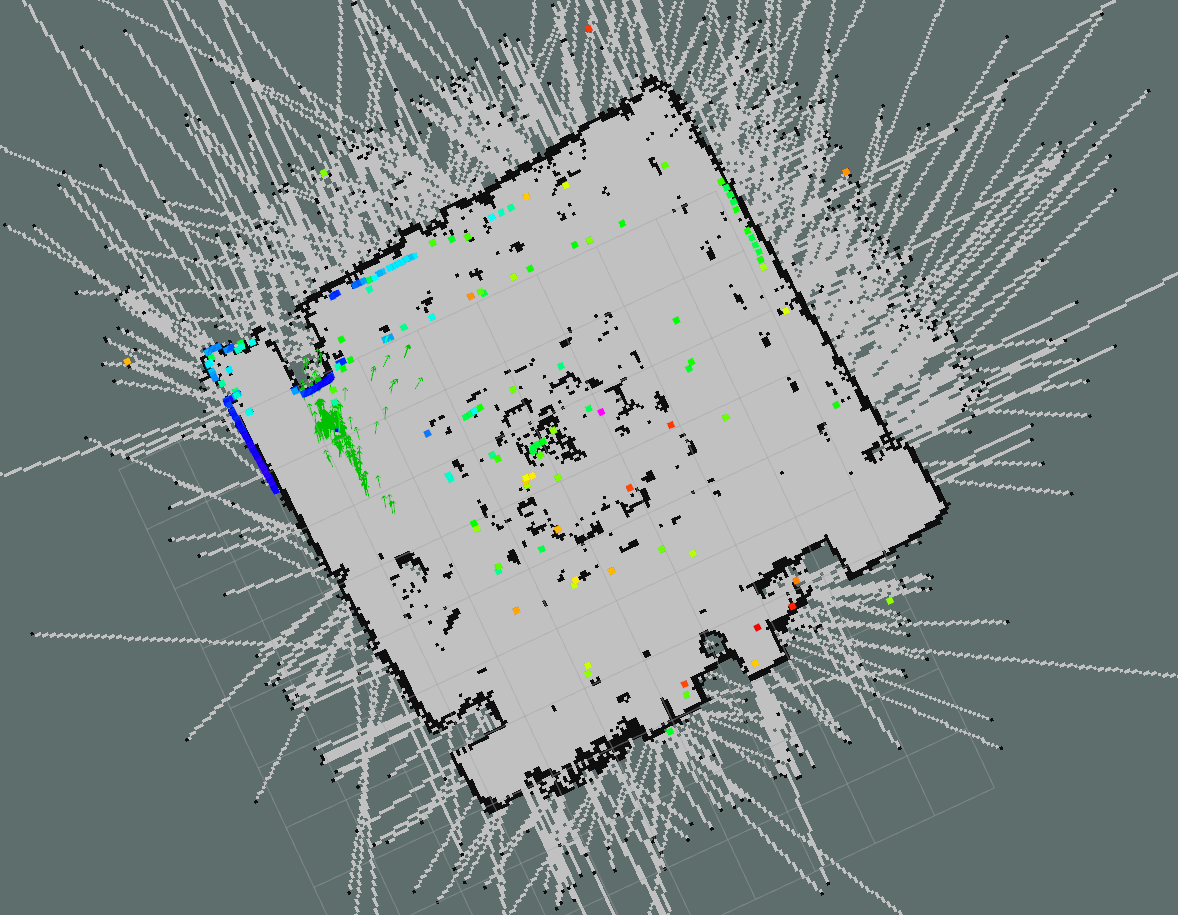
\includegraphics[width=0.7\linewidth, trim={4cm 5cm 12cm 6cm}, clip]{img/Experiment3_Lokalisierung_4.png}
\caption{Positionsschätzung bei Erreichen der Zielposition}
\end{figure}

Im letzten Schritt wird ein weiteres Navigationsziel gesetzt, woraufhin der Roboter sich weiter durch den Raum bewegt. Hier zeigt sich eine weitere Verdichtung der Partikelwolke, was sich darauf zurückführen lässt, dass die Distanzmessungen weiterhin mit der Karte übereinstimmen. Somit kann die Lokalisierung mit einem erhöhten Maß an Sicherheit als richtig angenommen werden.

An dieser Stelle sei eine negative Kopplung der Navigation und Lokalisierung erwähnt. Im Fall, dass die Lokalisierung in Form einer Positionsschätzung reinitialisiert wird und nur eine kurz entferntes Ziel angesteuert wird, wird während der Navigation die Position des Roboters durch den Lokalisierungsalgorithmus angepasst. Dies hat wiederum zur Folge, dass der Plan des Roboters überarbeitet werden muss, da die ursprüngliche Position verworfen wurde. Dies hat zur Folge, dass der Roboter wiederholte Rotationsmanöver ausführt, die von kurzen Translationsbewegung gefolgt werden. In diesem Muster bewegt sich der Roboter mehrere Male auf der Stelle, bis die Lokalisierung ein ausreichend hohes Maß an Sicherheit erreicht hat, sodass die geschätzte Position sich nur noch in einer für die Navigation nicht relevanten Größenordnung ändert.